
\chapter{Figures, Tables, and Pseudocode}
\label{ch:nontextelements}

Non-text elements such as figures, tables, and pseudocode play a crucial role in organizing the flow of the work.
By effectively using these components---in \LaTeX{}, via the use of so-called environments---, authors ensure an effective communication of their content.

% general

\guideline[g:nontext:refer_non_text_elements]
    {Refer to all non-text elements in the running text.}

\goodbadexample{
    ...
}{
    ...
}

\noindent The placement of non-text elements like figures, tables, and algorithms with respect to the running text is typically managed by \LaTeX{}, so readers often skip over them until a reference directs them to a specific element.
Therefore, it is good practice to explicitly reference each non-text element, ideally in a separate paragraph explaining its content.
% An alternative formulation to this guideline is:
% ``Only use environments if they are referenced at least once later.''


\guideline[g:nontext:placement_top]
    {Place non-text elements on the top of a page or column.}

\goodbadexample[{\cite[Sec.~II.B.]{Wetzlinger2025TAC}}]{
    \location{Top of the page} \\
    (...) \\
    The exact conversion from a polytope to a constrained zonotopes, denoted by $\textsc{CZ}(\mathcal{P})$, is computed using Algorithm 1, which implements [12, Thm. 1].
    
    \algruletop{}
\textbf{Algorithm 1} ~ Conversion: Polytope to constrained zonotope. \\
\textbf{Input:} Polytope $\mathcal{P} = \langle H, d \rangle_P$ \\
\textbf{Output:} Constrained zonotope $\mathcal{CZ} = \langle c, G, K, l \rangle_{CZ}$

\begin{algorithmic}[1]
	\State $\langle c, G \rangle_Z \gets \textsc{box}( \mathcal{P} )$
    \State $\forall j \in \mathbb{N}_{[1,...,h]}\colon o_{(j)} \gets -\rho\big( \langle c, G \rangle_Z,-H_{(j,\cdot)}^\top \big)$
    \State $G \gets [G \;\, \mathbf{0}]$, $K \gets [H G \;\, \tfrac{1}{2}\mathrm{diag}(o - d)]$, $l \gets \tfrac{1}{2}(d+o) - Hc$
    \State $\mathcal{CZ} \gets \langle c, G, K, l \rangle_{CZ}$
\end{algorithmic}
\algrulebottom{}


    The convex hull can be computed according to [13, Thm. 5] and the multiplication with an intervalmatrix $\mathbf{M}\mathcal{CZ}$ follows from (16).
}{
    \location{Top of the page} \\
    \algruletop{}
\textbf{Algorithm 1} ~ Conversion: Polytope to constrained zonotope. \\
\textbf{Input:} Polytope $\mathcal{P} = \langle H, d \rangle_P$ \\
\textbf{Output:} Constrained zonotope $\mathcal{CZ} = \langle c, G, K, l \rangle_{CZ}$

\begin{algorithmic}[1]
	\State $\langle c, G \rangle_Z \gets \textsc{box}( \mathcal{P} )$
    \State $\forall j \in \mathbb{N}_{[1,...,h]}\colon o_{(j)} \gets -\rho\big( \langle c, G \rangle_Z,-H_{(j,\cdot)}^\top \big)$
    \State $G \gets [G \;\, \mathbf{0}]$, $K \gets [H G \;\, \tfrac{1}{2}\mathrm{diag}(o - d)]$, $l \gets \tfrac{1}{2}(d+o) - Hc$
    \State $\mathcal{CZ} \gets \langle c, G, K, l \rangle_{CZ}$
\end{algorithmic}
\algrulebottom{}

    
    (...) \\
    The exact conversion from a polytope to a constrained zonotopes, denoted by $\textsc{CZ}(\mathcal{P})$, is computed using Algorithm 1, which implements [12, Thm. 1].
    The convex hull can be computed according to [13, Thm. 5] and the multiplication with an intervalmatrix $\mathbf{M}\mathcal{CZ}$ follows from (16).
}

\noindent Placing non-text elements at the top of the page or column offers several advantages:
First, these elements are easily accessible when referenced in the text.
Second, non-text elements often condense important information, warranting prominent placement, such as at the top of the page.
Third, this placement preserves the flow of the running text, contributing to optimizing space usage.

% figures

\guideline[g:nontext:figure_vector_graphics]
    {Figures: Use vector graphics.}

% bad: make bad screenshot of vector graphics
\goodbadexample{
    ...
}{
    ...
}

\noindent No exceptions.
Since figures typically capture the reader's attention first, investing in high-quality figures is well worth the effort.
Many applications offer the ability to export a drawn canvas as a vector graphics file.



\guideline[g:nontext:figure_same_font]
    {Figures: Use the same font and font sizes as in the running text.}

% bad: different font due to image generating program (or image screenshot, etc.)
\goodbadexample{
    ...
}{
    ...
}

\noindent Using the same font and font sizes in figures as in the running text allows the figure to blend seamlessly with the rest of the document, contributing to a cohesive overall appearance.
This is most easily achieved with the \LaTeX{} package \emph{TikZ}, as it compiles the text in figures using the same settings as the rest of the document.


\guideline[g:nontext:figure_colorvisiondeficiency]
    {Figures: Ensure colors are distinguishable.}

\goodbadexample[{\cite[Fig.~3]{Wetzlinger2023HSCC}}]{
    % This file was created by matlab2tikz.
%
%The latest updates can be retrieved from
%  http://www.mathworks.com/matlabcentral/fileexchange/22022-matlab2tikz-matlab2tikz
%where you can also make suggestions and rate matlab2tikz.
%
\definecolor{mycolor1}{rgb}{0.00000,0.36078,0.67059}%
\definecolor{mycolor2}{rgb}{0.89020,0.10588,0.13725}%

\tikzsetnextfilename{figure_cvd_bad}
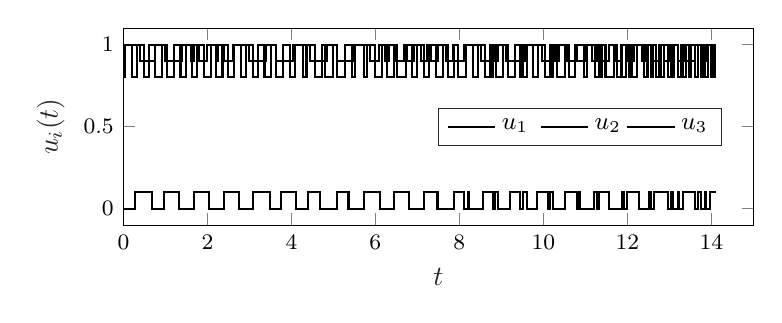
\begin{tikzpicture}

\begin{axis}[%
width=8cm,
height=2.5cm,
at={(0in,0in)},
scale only axis,
xmin=0.000,
xmax=15.000,
xlabel style={font=\color{white!15!black}},
xlabel={$t$},
ymin=-0.100,
ymax=1.100,
ylabel style={font=\color{white!15!black}},
ylabel={$u_i(t)$},
axis background/.style={fill=white},
legend columns = 3,
legend style={legend cell align=left, font=\small, align=left, draw=white!15!black,
	at={(0.95,0.5)}, anchor=east,
	/tikz/column 2/.style={column sep=0.075cm}},
%legend image post style={line width = 1pt},
every tick label/.append style={font=\footnotesize}
]

\addplot [color=black, line width=0.75pt]
  table[row sep=crcr]{%
0.000	0.000\\
0.280	0.000\\
0.280	0.100\\
0.680	0.100\\
0.680	0.000\\
0.960	0.000\\
0.960	0.100\\
1.320	0.100\\
1.320	0.000\\
1.680	0.000\\
1.680	0.100\\
2.040	0.100\\
2.040	0.000\\
2.400	0.000\\
2.400	0.100\\
2.760	0.100\\
2.760	0.000\\
3.080	0.000\\
3.080	0.100\\
3.480	0.100\\
3.480	0.000\\
3.760	0.000\\
3.760	0.100\\
4.120	0.100\\
4.120	0.000\\
4.400	0.000\\
4.400	0.100\\
4.680	0.100\\
4.680	0.000\\
5.080	0.000\\
5.080	0.100\\
5.360	0.100\\
5.360	0.000\\
5.720	0.000\\
5.720	0.100\\
6.120	0.100\\
6.120	0.000\\
6.440	0.000\\
6.440	0.100\\
6.800	0.100\\
6.800	0.000\\
7.160	0.000\\
7.160	0.100\\
7.480	0.100\\
7.480	0.000\\
7.880	0.000\\
7.880	0.100\\
8.120	0.100\\
8.120	0.000\\
8.200	0.000\\
8.200	0.100\\
8.240	0.100\\
8.240	0.000\\
8.560	0.000\\
8.560	0.100\\
8.800	0.100\\
8.800	0.000\\
8.840	0.000\\
8.840	0.100\\
8.920	0.100\\
8.920	0.000\\
9.200	0.000\\
9.200	0.100\\
9.440	0.100\\
9.440	0.000\\
9.520	0.000\\
9.520	0.100\\
9.600	0.100\\
9.600	0.000\\
9.840	0.000\\
9.840	0.100\\
10.120	0.100\\
10.120	0.000\\
10.160	0.000\\
10.160	0.100\\
10.240	0.100\\
10.240	0.000\\
10.520	0.000\\
10.520	0.100\\
10.800	0.100\\
10.800	0.000\\
10.840	0.000\\
10.840	0.100\\
10.880	0.100\\
10.880	0.000\\
11.200	0.000\\
11.200	0.100\\
11.280	0.100\\
11.280	0.000\\
11.320	0.000\\
11.320	0.100\\
11.560	0.100\\
11.560	0.000\\
11.880	0.000\\
11.880	0.100\\
11.920	0.100\\
11.920	0.000\\
12.000	0.000\\
12.000	0.100\\
12.280	0.100\\
12.280	0.000\\
12.520	0.000\\
12.520	0.100\\
12.560	0.100\\
12.560	0.000\\
12.640	0.000\\
12.640	0.100\\
12.960	0.100\\
12.960	0.000\\
13.040	0.000\\
13.040	0.100\\
13.080	0.100\\
13.080	0.000\\
13.200	0.000\\
13.200	0.100\\
13.240	0.100\\
13.240	0.000\\
13.320	0.000\\
13.320	0.100\\
13.600	0.100\\
13.600	0.000\\
13.680	0.000\\
13.680	0.100\\
13.760	0.100\\
13.760	0.000\\
13.840	0.000\\
13.840	0.100\\
13.880	0.100\\
13.880	0.000\\
13.960	0.000\\
13.960	0.100\\
14.120	0.100\\
};
\addlegendentry{$u_1$}

\addplot [color=black, line width=0.75pt]
  table[row sep=crcr]{%
0.000	0.800\\
0.040	0.800\\
0.040	1.000\\
0.200	1.000\\
0.200	0.800\\
0.320	0.800\\
0.320	1.000\\
0.480	1.000\\
0.480	0.800\\
0.600	0.800\\
0.600	1.000\\
0.760	1.000\\
0.760	0.800\\
0.920	0.800\\
0.920	1.000\\
1.040	1.000\\
1.040	0.800\\
1.200	0.800\\
1.200	1.000\\
1.360	1.000\\
1.360	0.800\\
1.480	0.800\\
1.480	1.000\\
1.640	1.000\\
1.640	0.800\\
1.760	0.800\\
1.760	1.000\\
1.920	1.000\\
1.920	0.800\\
2.080	0.800\\
2.080	1.000\\
2.200	1.000\\
2.200	0.800\\
2.360	0.800\\
2.360	1.000\\
2.480	1.000\\
2.480	0.800\\
2.640	0.800\\
2.640	1.000\\
2.800	1.000\\
2.800	0.800\\
2.920	0.800\\
2.920	1.000\\
3.080	1.000\\
3.080	0.800\\
3.200	0.800\\
3.200	1.000\\
3.360	1.000\\
3.360	0.800\\
3.520	0.800\\
3.520	1.000\\
3.640	1.000\\
3.640	0.800\\
3.800	0.800\\
3.800	1.000\\
3.960	1.000\\
3.960	0.800\\
4.080	0.800\\
4.080	1.000\\
4.280	1.000\\
4.280	0.800\\
4.360	0.800\\
4.360	1.000\\
4.560	1.000\\
4.560	0.800\\
4.720	0.800\\
4.720	1.000\\
4.800	1.000\\
4.800	0.800\\
5.000	0.800\\
5.000	1.000\\
5.080	1.000\\
5.080	0.800\\
5.280	0.800\\
5.280	1.000\\
5.440	1.000\\
5.440	0.800\\
5.520	0.800\\
5.520	1.000\\
5.720	1.000\\
5.720	0.800\\
5.800	0.800\\
5.800	1.000\\
6.000	1.000\\
6.000	0.800\\
6.160	0.800\\
6.160	1.000\\
6.280	1.000\\
6.280	0.800\\
6.440	0.800\\
6.440	1.000\\
6.520	1.000\\
6.520	0.800\\
6.720	0.800\\
6.720	1.000\\
6.880	1.000\\
6.880	0.800\\
7.000	0.800\\
7.000	1.000\\
7.160	1.000\\
7.160	0.800\\
7.280	0.800\\
7.280	1.000\\
7.440	1.000\\
7.440	0.800\\
7.600	0.800\\
7.600	1.000\\
7.720	1.000\\
7.720	0.800\\
7.880	0.800\\
7.880	1.000\\
7.960	1.000\\
7.960	0.800\\
8.160	0.800\\
8.160	1.000\\
8.320	1.000\\
8.320	0.800\\
8.440	0.800\\
8.440	1.000\\
8.600	1.000\\
8.600	0.800\\
8.720	0.800\\
8.720	1.000\\
8.760	1.000\\
8.760	0.800\\
8.800	0.800\\
8.800	1.000\\
8.880	1.000\\
8.880	0.800\\
9.040	0.800\\
9.040	1.000\\
9.160	1.000\\
9.160	0.800\\
9.320	0.800\\
9.320	1.000\\
9.440	1.000\\
9.440	0.800\\
9.480	0.800\\
9.480	1.000\\
9.520	1.000\\
9.520	0.800\\
9.600	0.800\\
9.600	1.000\\
9.760	1.000\\
9.760	0.800\\
9.880	0.800\\
9.880	1.000\\
10.040	1.000\\
10.040	0.800\\
10.160	0.800\\
10.160	1.000\\
10.200	1.000\\
10.200	0.800\\
10.240	0.800\\
10.240	1.000\\
10.320	1.000\\
10.320	0.800\\
10.520	0.800\\
10.520	1.000\\
10.600	1.000\\
10.600	0.800\\
10.760	0.800\\
10.760	1.000\\
10.960	1.000\\
10.960	0.800\\
11.040	0.800\\
11.040	1.000\\
11.240	1.000\\
11.240	0.800\\
11.320	0.800\\
11.320	1.000\\
11.360	1.000\\
11.360	0.800\\
11.400	0.800\\
11.400	1.000\\
11.480	1.000\\
11.480	0.800\\
11.680	0.800\\
11.680	1.000\\
11.760	1.000\\
11.760	0.800\\
11.840	0.800\\
11.840	1.000\\
11.880	1.000\\
11.880	0.800\\
11.960	0.800\\
11.960	1.000\\
12.040	1.000\\
12.040	0.800\\
12.080	0.800\\
12.080	1.000\\
12.120	1.000\\
12.120	0.800\\
12.240	0.800\\
12.240	1.000\\
12.400	1.000\\
12.400	0.800\\
12.480	0.800\\
12.480	1.000\\
12.560	1.000\\
12.560	0.800\\
12.600	0.800\\
12.600	1.000\\
12.680	1.000\\
12.680	0.800\\
12.760	0.800\\
12.760	1.000\\
12.800	1.000\\
12.800	0.800\\
12.880	0.800\\
12.880	1.000\\
12.960	1.000\\
12.960	0.800\\
13.040	0.800\\
13.040	1.000\\
13.080	1.000\\
13.080	0.800\\
13.120	0.800\\
13.120	1.000\\
13.200	1.000\\
13.200	0.800\\
13.280	0.800\\
13.280	1.000\\
13.320	1.000\\
13.320	0.800\\
13.400	0.800\\
13.400	1.000\\
13.480	1.000\\
13.480	0.800\\
13.520	0.800\\
13.520	1.000\\
13.600	1.000\\
13.600	0.800\\
13.680	0.800\\
13.680	1.000\\
13.760	1.000\\
13.760	0.800\\
13.800	0.800\\
13.800	1.000\\
13.840	1.000\\
13.840	0.800\\
13.920	0.800\\
13.920	1.000\\
14.000	1.000\\
14.000	0.800\\
14.040	0.800\\
14.040	1.000\\
14.080	1.000\\
14.080	0.800\\
14.120	0.800\\
};
\addlegendentry{$u_2$}

\addplot [color=black, line width=0.75pt]
  table[row sep=crcr]{%
0.000	1.000\\
0.400	1.000\\
0.400	0.900\\
0.760	0.900\\
0.760	1.000\\
1.000	1.000\\
1.000	0.900\\
1.400	0.900\\
1.400	1.000\\
1.600	1.000\\
1.600	0.900\\
1.680	0.900\\
1.680	1.000\\
1.800	1.000\\
1.800	0.900\\
2.000	0.900\\
2.000	1.000\\
2.200	1.000\\
2.200	0.900\\
2.240	0.900\\
2.240	1.000\\
2.400	1.000\\
2.400	0.900\\
2.600	0.900\\
2.600	1.000\\
3.000	1.000\\
3.000	0.900\\
3.400	0.900\\
3.400	1.000\\
3.640	1.000\\
3.640	0.900\\
4.040	0.900\\
4.040	1.000\\
4.440	1.000\\
4.440	0.900\\
4.840	0.900\\
4.840	1.000\\
5.080	1.000\\
5.080	0.900\\
5.480	0.900\\
5.480	1.000\\
5.880	1.000\\
5.880	0.900\\
6.080	0.900\\
6.080	1.000\\
6.240	1.000\\
6.240	0.900\\
6.320	0.900\\
6.320	1.000\\
6.480	1.000\\
6.480	0.900\\
6.680	0.900\\
6.680	1.000\\
6.760	1.000\\
6.760	0.900\\
6.920	0.900\\
6.920	1.000\\
7.080	1.000\\
7.080	0.900\\
7.240	0.900\\
7.240	1.000\\
7.320	1.000\\
7.320	0.900\\
7.480	0.900\\
7.480	1.000\\
7.680	1.000\\
7.680	0.900\\
7.840	0.900\\
7.840	1.000\\
7.880	1.000\\
7.880	0.900\\
8.120	0.900\\
8.120	1.000\\
8.520	1.000\\
8.520	0.900\\
8.760	0.900\\
8.760	1.000\\
8.840	1.000\\
8.840	0.900\\
8.920	0.900\\
8.920	1.000\\
9.120	1.000\\
9.120	0.900\\
9.560	0.900\\
9.560	1.000\\
9.960	1.000\\
9.960	0.900\\
10.160	0.900\\
10.160	1.000\\
10.280	1.000\\
10.280	0.900\\
10.360	0.900\\
10.360	1.000\\
10.560	1.000\\
10.560	0.900\\
10.760	0.900\\
10.760	1.000\\
10.800	1.000\\
10.800	0.900\\
11.000	0.900\\
11.000	1.000\\
11.160	1.000\\
11.160	0.900\\
11.280	0.900\\
11.280	1.000\\
11.400	1.000\\
11.400	0.900\\
11.560	0.900\\
11.560	1.000\\
11.720	1.000\\
11.720	0.900\\
11.880	0.900\\
11.880	1.000\\
12.000	1.000\\
12.000	0.900\\
12.160	0.900\\
12.160	1.000\\
12.360	1.000\\
12.360	0.900\\
12.440	0.900\\
12.440	1.000\\
12.600	1.000\\
12.600	0.900\\
12.800	0.900\\
12.800	1.000\\
12.880	1.000\\
12.880	0.900\\
13.000	0.900\\
13.000	1.000\\
13.200	1.000\\
13.200	0.900\\
13.360	0.900\\
13.360	1.000\\
13.400	1.000\\
13.400	0.900\\
13.600	0.900\\
13.600	1.000\\
13.840	1.000\\
13.840	0.900\\
13.880	0.900\\
13.880	1.000\\
14.000	1.000\\
14.000	0.900\\
14.120	0.900\\
};
\addlegendentry{$u_3$}

\end{axis}

\end{tikzpicture}

    \badexpl{We use only black lines to simulate how indistinguishable colors can appear to individuals with color vision deficiency.}
}{
    \input{data/figure_cvd_good.tikz}
}

\noindent
Color vision deficiency affects approximately $8\%$ of men and $0.5\%$ of women worldwide, or roughly $1$ in $12$ men and $1$ in $200$ women \footfullcite{Gordon1998}.
As a result, it is highly likely that some readers would benefit from color choices that accommodate this condition.


\guideline[g:nontext:figure_linestyles]
    {Figures: Consider using different line styles.}

\goodbadexample[{\cite[Fig.~3]{Wetzlinger2024CSL}}]{
    \input{data/figure_linestyle_bad.tikz}
}{
    % This file was created by matlab2tikz.
%
%The latest updates can be retrieved from
%  http://www.mathworks.com/matlabcentral/fileexchange/22022-matlab2tikz-matlab2tikz
%where you can also make suggestions and rate matlab2tikz.
%
\definecolor{mycolor1}{rgb}{0.00000,0.36078,0.67059}%
\definecolor{mycolor2}{rgb}{0.89020,0.10588,0.13725}%
%
\tikzsetnextfilename{figure_cvd_good}
\begin{tikzpicture}

\begin{axis}[%
width=7.5cm,
height=3.1cm,
at={(0in,0in)},
scale only axis,
xmin=0.000,
xmax=3.000,
xlabel style={font=\color{white!15!black}},
xlabel={$t$},
ymin=0.000,
ymax=1.000,
ylabel style={font=\color{white!15!black}},
ylabel={$\gamma_{\min}(t)$},
axis background/.style={fill=white},
legend columns = 3,
legend style={legend cell align=left, font=\small, align=left, draw=white!15!black,
	at={(-0.1,-0.4)}, anchor=north west,
	/tikz/column 2/.style={column sep=0.075cm}},
%legend image post style={line width = 1pt},
every tick label/.append style={font=\footnotesize}
]

\addplot [color=mycolor1, line width=1pt]
  table[row sep=crcr]{%
0	1\\
0.01	0.995\\
0.02	0.991\\
0.05	0.976\\
0.06	0.972\\
0.08	0.962\\
0.09	0.958\\
0.11	0.948\\
0.12	0.944\\
0.14	0.934\\
0.15	0.93\\
0.16	0.925\\
0.17	0.921\\
0.18	0.916\\
0.2	0.908\\
0.21	0.903\\
0.29	0.871\\
0.3	0.868\\
0.31	0.864\\
0.33	0.858\\
0.34	0.854\\
0.38	0.842\\
0.39	0.84\\
0.4	0.837\\
0.41	0.835\\
0.42	0.832\\
0.47	0.822\\
0.48	0.821\\
0.49	0.819\\
0.53	0.815\\
0.54	0.815\\
0.55	0.814\\
0.56	0.814\\
0.58	0.812\\
0.59	0.812\\
0.61	0.81\\
0.62	0.81\\
0.63	0.809\\
0.65	0.809\\
0.66	0.808\\
0.69	0.808\\
0.75	0.796\\
0.76	0.795\\
0.77	0.793\\
0.78	0.792\\
0.8	0.788\\
0.81	0.787\\
0.82	0.785\\
0.83	0.784\\
0.84	0.782\\
0.86	0.78\\
0.87	0.778\\
0.88	0.777\\
0.89	0.775\\
0.91	0.773\\
0.92	0.771\\
0.96	0.767\\
0.97	0.765\\
1.04	0.758\\
1.05	0.758\\
1.08	0.755\\
1.09	0.755\\
1.13	0.751\\
1.14	0.751\\
1.17	0.748\\
1.18	0.748\\
1.21	0.745\\
1.22	0.745\\
1.23	0.744\\
1.24	0.744\\
1.25	0.743\\
1.26	0.743\\
1.27	0.742\\
1.28	0.742\\
1.29	0.741\\
1.3	0.741\\
1.31	0.74\\
1.32	0.74\\
1.33	0.739\\
1.34	0.739\\
1.35	0.738\\
1.36	0.738\\
1.37	0.737\\
1.39	0.737\\
1.4	0.736\\
1.42	0.736\\
1.43	0.735\\
1.45	0.735\\
1.46	0.734\\
1.49	0.734\\
1.5	0.733\\
1.56	0.733\\
1.57	0.732\\
1.6	0.732\\
1.61	0.731\\
1.62	0.731\\
1.63	0.73\\
1.64	0.73\\
1.67	0.727\\
1.68	0.727\\
1.7	0.725\\
1.71	0.725\\
1.72	0.724\\
1.73	0.724\\
1.74	0.723\\
1.76	0.723\\
1.78	0.711\\
1.79	0.704\\
1.8	0.704\\
1.81	0.703\\
1.82	0.697\\
1.86	0.669\\
1.87	0.661\\
1.88	0.64\\
1.89	0.614\\
1.91	0.564\\
1.92	0.548\\
1.93	0.571\\
1.94	0.591\\
1.95	0.607\\
1.96	0.621\\
1.97	0.633\\
1.98	0.641\\
1.99	0.647\\
2	0.645\\
2.02	0.631\\
2.03	0.623\\
2.04	0.618\\
2.07	0.612\\
2.09	0.606\\
2.1	0.604\\
2.11	0.6\\
2.12	0.597\\
2.16	0.581\\
2.2	0.561\\
2.24	0.537\\
2.25	0.532\\
2.28	0.514\\
2.29	0.509\\
2.3	0.503\\
2.31	0.498\\
2.32	0.492\\
2.36	0.472\\
2.37	0.468\\
2.38	0.463\\
2.4	0.455\\
2.41	0.45\\
2.42	0.446\\
2.43	0.443\\
2.45	0.435\\
2.47	0.429\\
2.48	0.425\\
2.49	0.422\\
2.5	0.42\\
2.52	0.414\\
2.54	0.41\\
2.55	0.407\\
2.57	0.403\\
2.58	0.4\\
2.6	0.396\\
2.61	0.393\\
2.62	0.391\\
2.63	0.388\\
2.65	0.384\\
2.66	0.381\\
2.68	0.377\\
2.69	0.374\\
2.73	0.366\\
2.74	0.363\\
2.84	0.343\\
2.85	0.342\\
2.89	0.334\\
2.9	0.333\\
2.92	0.329\\
2.93	0.328\\
2.95	0.324\\
2.96	0.323\\
2.97	0.321\\
2.98	0.32\\
2.99	0.318\\
3	0.317\\
3	0\\
};
\addlegendentry{Algorithm 1}

\addplot [color=mycolor2, dashed, line width=1pt]
  table[row sep=crcr]{%
0	1.000\\
0.02	0.851\\
0.03	0.853\\
0.04	0.854\\
0.05	0.854\\
0.06	0.855\\
0.08	0.855\\
0.09	0.856\\
0.1	0.856\\
0.11	0.857\\
0.13	0.857\\
0.14	0.858\\
0.16	0.858\\
0.17	0.859\\
0.19	0.859\\
0.2	0.86\\
0.22	0.86\\
0.23	0.861\\
0.26	0.861\\
0.27	0.862\\
0.32	0.862\\
0.33	0.863\\
0.41	0.863\\
0.42	0.862\\
0.46	0.862\\
0.47	0.861\\
0.48	0.861\\
0.49	0.86\\
0.5	0.861\\
0.51	0.861\\
0.52	0.862\\
0.53	0.862\\
0.54	0.863\\
0.55	0.863\\
0.56	0.864\\
0.57	0.864\\
0.58	0.863\\
0.6	0.863\\
0.61	0.862\\
0.62	0.862\\
0.63	0.863\\
0.64	0.865\\
0.65	0.866\\
0.67	0.87\\
0.68	0.871\\
0.69	0.873\\
0.7	0.872\\
0.71	0.872\\
0.72	0.871\\
0.73	0.871\\
0.74	0.87\\
0.75	0.87\\
0.76	0.869\\
0.8	0.869\\
0.82	0.867\\
0.83	0.865\\
0.84	0.865\\
0.87	0.862\\
0.88	0.86\\
0.89	0.86\\
0.9	0.858\\
0.92	0.856\\
0.93	0.854\\
0.94	0.853\\
0.95	0.853\\
0.97	0.849\\
0.98	0.848\\
0.99	0.846\\
1	0.845\\
1.01	0.843\\
1.03	0.841\\
1.04	0.839\\
1.05	0.841\\
1.06	0.837\\
1.07	0.835\\
1.08	0.834\\
1.09	0.832\\
1.1	0.831\\
1.11	0.831\\
1.12	0.827\\
1.13	0.826\\
1.16	0.82\\
1.17	0.819\\
1.26	0.801\\
1.27	0.8\\
1.28	0.798\\
1.3	0.792\\
1.34	0.784\\
1.35	0.781\\
1.37	0.777\\
1.38	0.774\\
1.4	0.77\\
1.41	0.767\\
1.42	0.765\\
1.43	0.767\\
1.44	0.759\\
1.45	0.757\\
1.47	0.751\\
1.49	0.747\\
1.5	0.744\\
1.51	0.74\\
1.53	0.736\\
1.56	0.727\\
1.58	0.719\\
1.59	0.717\\
1.6	0.712\\
1.61	0.709\\
1.62	0.705\\
1.64	0.695\\
1.65	0.692\\
1.69	0.668\\
1.7	0\\
1.72	0\\
1.73	0.637\\
1.74	0.63\\
1.75	0\\
3	0\\
};
\addlegendentry{Approach in [10]}

\addplot [color=black, dashdotted, line width=1pt]
  table[row sep=crcr]{%
0	1\\
0.03	0.988\\
0.04	0.983\\
0.07	0.971\\
0.08	0.966\\
0.09	0.962\\
0.11	0.952\\
0.12	0.948\\
0.14	0.938\\
0.15	0.934\\
0.27	0.874\\
0.28	0.868\\
0.32	0.848\\
0.33	0.842\\
0.35	0.832\\
0.36	0.826\\
0.38	0.816\\
0.39	0.81\\
0.4	0.805\\
0.41	0.799\\
0.42	0.794\\
0.43	0.788\\
0.44	0.783\\
0.46	0.771\\
0.47	0.766\\
0.48	0.76\\
0.49	0.755\\
0.5	0.749\\
0.51	0.744\\
0.52	0.738\\
0.53	0.733\\
0.54	0.727\\
0.55	0.722\\
0.58	0.704\\
0.59	0.697\\
0.6	0.691\\
0.61	0.684\\
0.64	0.666\\
0.65	0.661\\
0.67	0.649\\
0.68	0.644\\
0.69	0.638\\
0.75	0.596\\
0.76	0.59\\
0.78	0.576\\
0.79	0.57\\
0.8	0.563\\
0.81	0.557\\
0.82	0.55\\
0.91	0.496\\
0.92	0.491\\
0.94	0.483\\
0.95	0.478\\
1	0.458\\
1.01	0.455\\
1.03	0.447\\
1.04	0.444\\
1.06	0.436\\
1.07	0.433\\
1.08	0.429\\
1.1	0.423\\
1.11	0.419\\
1.12	0.416\\
1.13	0.412\\
1.15	0.406\\
1.16	0.402\\
1.19	0.393\\
1.2	0.389\\
1.3	0.359\\
1.31	0.357\\
1.36	0.342\\
1.37	0.34\\
1.39	0.334\\
1.4	0.332\\
1.42	0.326\\
1.43	0.324\\
1.44	0.321\\
1.45	0.319\\
1.46	0.316\\
1.47	0.314\\
1.48	0.311\\
1.49	0.309\\
1.5	0.306\\
1.51	0.304\\
1.53	0.298\\
1.55	0.294\\
1.56	0.291\\
1.57	0.29\\
1.58	0.288\\
1.6	0.286\\
1.61	0.284\\
1.64	0.281\\
1.65	0.279\\
1.73	0.271\\
1.74	0.271\\
1.75	0.27\\
1.76	0.27\\
1.77	0.269\\
1.78	0.269\\
1.79	0.268\\
1.84	0.268\\
1.85	0.27\\
1.87	0.28\\
1.9	0.298\\
1.91	0.301\\
1.93	0.287\\
1.95	0.269\\
1.97	0.247\\
1.99	0.223\\
2.01	0.197\\
2.02	0.187\\
2.04	0.173\\
2.05	0.167\\
2.06	0.16\\
2.11	0.13\\
2.12	0.136\\
2.14	0.146\\
2.17	0.158\\
2.19	0.164\\
2.2	0.166\\
2.21	0.169\\
2.22	0.137\\
2.23	0.097\\
2.24	0.054\\
2.25	0.009\\
2.26	0\\
3	0\\
};
\addlegendentry{Approach in [5]}

\end{axis}

\end{tikzpicture}%
}

\noindent Varying line styles help differentiate information, making figures more accessible and easier to interpret.
Additionally, line styles are easier to reference in the caption and the running text, as colors may appear differently in black-and-white prints.


\guideline[g:nontext:figure_caption]
    {Figures: Captions should provide a brief, independent summary.}

% bad: caption that does not fully explain what is going on
% note: some parts may be explained by the legend, too
\goodbadexample{
    ...
}{
    ...
}

\noindent A good caption provides a concise description of the figure's content, enabling it to be understood without reference to the running text.
To achieve this, all objects, lines, and shading should be clearly explained.

% tables

\guideline[g:nontext:table_horizontal_lines]
    {Tables: Avoid horizontal lines.}

\goodbadexample{
    ...
}{
    ...
}

\noindent Excessive use of horizontal lines can make a table look cluttered and hinder the reader's ability to quickly scan and interpret the data, as the structure provided by rows and columns is often enough to visually separate data.
Horizontal lines are primarily used for sectioning, e.g., between column headers and data, or between different segments of similar data.


\guideline[g:nontext:table_highlight_bold]
    {Tables: Highlight the best results in bold.}

\goodbadexample[Adapted from {\cite[Tab.~I]{Wetzlinger2024CSL}}]{
    % \begin{small}
% Table I: Comparison of Algorithm 1 with the approaches [5], [10] in terms of computation time (in $\SI{}{\second}$) and tightness metric $\gamma_{\min}(t_{\normalfont\text{end}})$ (26).
% \end{small}

% \smallskip

\begin{footnotesize}
\begin{tabular}{l c c c c c c}
    \toprule
    \multirow{2}{*}{\textbf{Benchmark}} & \multirow{2}{*}{$\cdots$} & \multicolumn{2}{c}{\textbf{Algorithm 1}} & \multicolumn{2}{c}{\textbf{Scaling approach~[10]}} & \multirow{2}{*}{$\cdots$} \\
    & & Time & $\gamma_{\min}(t_{\text{end}})$ & Time & $\gamma_{\min}(t_{\text{end}})$ & \\ \midrule
    Jet Engine & & $3.9$ & $0.7769$ & $40$ & $0.6093$ & \\
    Higgins-Selkov & & $2.5$ & $0.8505$ & $57$ & $0.5896$ & \\
    Rössler & & $1.1$ & $0.7335$ & $32$ & $0.7137$ & \\
    Lotka-Volterra & & $0.99$ & $0.7711$ & $238$ & $0.8240$ & \\
    Biological model & & $0.59$ & $0.7540$ & $82$ & $0.8760$ & \\
    \bottomrule
\end{tabular}
\end{footnotesize}
}{
    \input{data/table_boldface_good.tex}
}

\noindent
Highlighting the best values adds a layer of visual hierarchy to the table, helping readers more easily compare the results.
Furthermore, this visual aid also facilitates a simpler discussion the results, as multiple bold entries clearly suggest strong performance.


\guideline[g:nontext:table_caption]
    {Tables: Explain all variables used in the caption.}

\newpage

\goodexample[Adapted from {\cite[Tab.~I]{Wetzlinger2025TAC}}]{
    \begin{small}
Table I: Runtime complexity of set operations for $n$-dimensional sets: \highlightpart{The polytope $\mathcal{P}$ has $h \geq n \in \mathbb{N}$ constraints, the constrained zonotope $\mathcal{CZ}$ and the zonotope $\mathcal{Z}$ have $\gamma \geq n \in \mathbb{N}$ generators, $\ell \in \mathbb{R}^n$ is a vector, and $\textsc{SF}(\mathcal{S})$ denotes the runtime complexity to evaluate $\rho(\mathcal{S},\ell)$.}
\end{small}

\begin{center}
\begin{footnotesize}
\begin{tabular}{l l c l l}
	\toprule
	\textbf{Operation} & \textbf{Complexity} & & \textbf{Operation} & \textbf{Complexity} \\ \cmidrule{1-2} \cmidrule{4-5}
	$M \mathcal{P}$ & $\mathcal{O}(hn^2)$
		& & $\mathcal{Z}_1 \oplus \mathcal{Z}_2$ & $\mathcal{O}(n)$ \\
	$M\mathcal{Z}$ & $\mathcal{O}(n^2\gamma)$
	    & & $\mathcal{CZ}_1 \! \oplus \mathcal{CZ}_2$ & $\mathcal{O}(n)$ \\
	$M \mathcal{CZ}$ & $\mathcal{O}(n^2\gamma)$
		& & $\mathcal{P} \ominus \mathcal{S}$ & $\mathcal{O}(h \textsc{SF}(\mathcal{S}))$ \\
	$\mathbf{M} \mathcal{Z}$ & $\mathcal{O}(n^2\gamma)$
	    & & $\mathcal{S} \subseteq \mathcal{P}$ & $\mathcal{O}(h \textsc{SF}(\mathcal{S}))$ \\
	$\mathbf{M}\mathcal{CZ}$ & $\mathcal{O}(n^2\gamma)$
	    & & $\mathcal{CZ} \cap \mathcal{P}$ & $\mathcal{O}(h\gamma^{3.5})$ \\
	$\rho(\mathcal{P},\ell)$ & $\mathcal{O}(h^{3.5})$
	    & & $\textsc{conv}(\mathcal{CZ}_1,\mathcal{CZ}_2)$ & $\mathcal{O}(n)$ \\
	$\rho(\mathcal{Z},\ell)$ & $\mathcal{O}(n\gamma)$
		& & $\textsc{box}(\mathcal{P})$ & $\mathcal{O}(nh^{3.5})$ \\
	$\rho(\mathcal{CZ},\ell)$ & $\mathcal{O}(\gamma^{3.5})$
		& & $\textsc{CZ}(\mathcal{P})$ & $\mathcal{O}(nh^{3.5})$ \\
	\bottomrule
\end{tabular}
\end{footnotesize}
\end{center}

}

\noindent
To enable readers to understand the table independently of the running text, concisely describe all used variables in the caption, even if their meaning is consistent throughout the paper.
This explanation usually comes after a brief summary of the table's content.

% pseudocode

\guideline[g:nontext:pseudocode_language_specific]
    {Avoid language-specific functions in pseudocode.}

\goodbadexample{
    \algruletop{}
\textbf{Algorithm 1.} A good algorithm. \\
\textbf{Input}: Matrix $G$, (...) \\
\textbf{Output}: (...) \\
\begin{scriptsize}
    1:
\end{scriptsize}
$m \gets \highlightpartmath{\textsc{shape}(G,2)}$ \\
(...) \\
\algrulebottom{}
}{
    \algruletop{}
\textbf{Algorithm 1.} A good algorithm. \\
\textbf{Input}: Matrix $G \in \mathbb{R}^{n \times \highlightpartmath{m}}$, (...) \\
\textbf{Output}: (...) \\
(...) \\
\algrulebottom{}
}

\noindent
Using language-specific functions may hinder understanding across different audiences, as some readers may not be familiar with the used programming language.
In simple cases, there may be a mathematical alternative to achieve the same goal.
If a language-specific function is particularly useful, briefly describe its behavior in the running text.


\guideline[g:nontext:pseudocode_explain_operators]
    {Pseudocode: Ensure that all operators are explained or referenced.}

% same example, bad one relies on "context understanding", good one explicitly explains the operators
\goodbadexample{
    ...
}{
    ...
}

\noindent Since pseudocode aims to be concise, it's often better to use named operations rather than detailing every computation, especially for standard tasks, e.g., sorting.
However, it is still good practice to briefly explain what each operation does, particularly in terms of its input and output arguments.


\guideline[g:nontext:pseudocode_io_arguments]
    {Pseudocode: Strictly define the input and output arguments.}

\goodexample[Adapted from {\cite[Alg.~1]{Wetzlinger2024CSL}}]{
    \algruletop{}
\textbf{Algorithm 1} ~ Inner approximation of the reachable set \\
\highlightpart{\textbf{Require:} Nonlinear system $\dot{x}(t) = f(x(t))$,
polytopic initial set $\mathcal{X}_0 = \langle H, d \rangle_H$, time horizon $\tau = [0,t_{\text{end}}]$, steps $\omega \in \mathbb{N}$}

\highlightpart{\textbf{Ensure:} Inner approximation of the reachable set $\widecheck{\mathcal{R}}(\tau)$}

\begin{algorithmic}[1]
	\State (...)
\end{algorithmic}
\algrulebottom{}

}

\noindent
A clear definition of input arguments makes the assumptions made by the algorithm transparent.
It also helps those re-implementing a specific pseudocode.

